\section{Personal}

El presente OCD propone un sistema en el que el factor humano tiene la mayor parte de responsabilidad en el funcionamiento del mismo. Por consiguiente, será el factor humano el encargado de supervisar y controlar el espacio aéreo. Se encargará también de controlar los sistemas, siendo el factor humano el que debe tomar la última decisión. Por último, deberá proponer iniciativas para mejorar su funcionamiento.

\subsection{Estructura Organizacional}

En los siguientes apartados se detallan las distintas posiciones que componen la estructura organizacional con sus roles, tareas y responsabilidades. Dado que el presente OCD ubica el factor humano en el centro del sistema otorgándole una relevancia absoluta en las decisiones que se toman, todos las cargos siguientes van a desempeñar un papel fundamental en el funcionamiento del sistema. En la figura () se puede observar el organigrama que resume la estructura propuesta.

\begin{figure}[H]
    \centering
    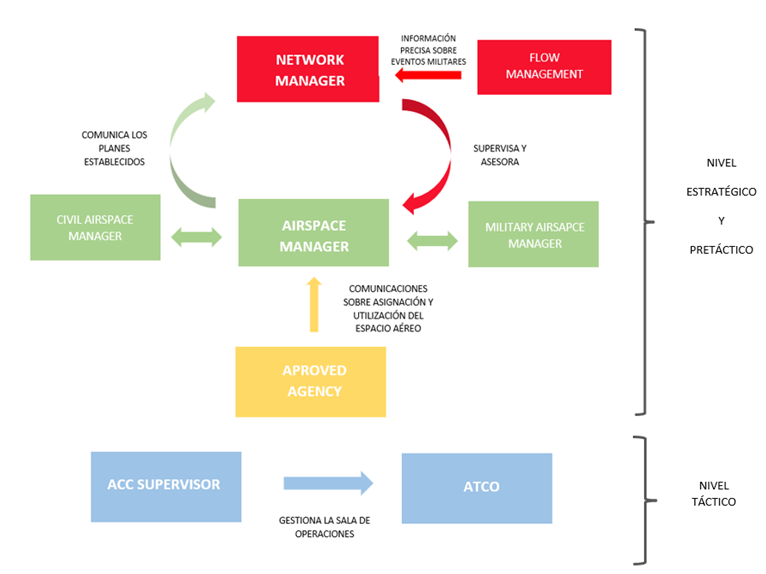
\includegraphics[width=1\linewidth]{figuras/estructura.png}
    \caption{Organigrama propuesto.}
    \label{fig:estructura}
\end{figure}

\subsubsection{Network Manager (NM)}

Actúa como catalizador y facilitador para una gestión general de la red eficiente por parte de todas las partes interesadas de el ATM. Pertenece al primer nivel de gestión, planificación estratégica, definido en el apartado (\ref{tit:level1}).
    
\begin{itemize}
    \item Tiene un papel clave en la fase de planificación a largo plazo para garantizar el rendimiento eficiente de la Red.
    
    \item Supervisa todas las actividades locales o subregionales a largo plazo e identifica las situaciones en las que el rendimiento puede verse afectado.
    
    \item Se encarga de coordinar toda la organizaciones responsables de las decisiones de alto nivel para garantizar la coherencia de las operaciones de la Red. Asesora a estas organizaiones de nivel nacional y subregional.
    
    \item Prepara la planificación estacional o los planes para eventos especiales.
    
    \item Es el responsable de la creación, publicación y mantenimiento del \acrfull{nop}.
\end{itemize}

\subsubsection{Airspace Manager (AM)}

El Airspace Manager se centra en la fases de planificación a medio y corto plazo. Corresponde al nivel 2 de gestión, pre-táctico, visto en el apartado (\ref{tit:level2}). Se encuentra ubicado en el ámbito nacional y/o subregional. 

\begin{itemize}
    \item Su principal función es la planificación a medio y corto plazo de las operaciones.
    
    \item La tarea del AM es gestionar las demandas de espacio aéreo de las operaciones civiles y militares de una manera pragmática, teniendo en cuenta los factores pertinentes.
    
    \item El papel del AM en la práctica será desempeñado por dos actores: el Civil Airspace Manager  (CAM) y el Military  Airspace  Manager (MAM), estos actores tendrían entonces funciones y áreas de autoridad claramente definidas a nivel local.
    
    \item Se encargará de la gestión de las CDR, las restricción por ejercicios militares y la asignación de espacio aéreo. 
    
    \item Se encargará de diseñar y publicar los \acrfull{aup} y los \acrfull{uup}.
    
    \item Comunica al NM los planes establecidos.
\end{itemize}

\subsubsection{ACC Supervisor}    

Se puesto se encuentra en la sala de operaciones y participa en la toma de decisiones en tiempo real.

\begin{itemize}
    \item Se encarga de gestionar todas las actividades de la sala de operaciones, decidiendo las posiciones de trabajo que deben ocupar los controladores de acuerdo a la demanda esperada.
    
    \item También se encarga de tomar decisiones relativas a la configuración de los diferentes sectores para ajustar la capacidad a la demanda. Los resultados de las simulaciones pueden implementarse por parte del \acrfull{atfcm} a través del \acrfull{cdm}.
    
    \item Por el lado militar, la figura corresponde a la función del ATC Military Supervisor role. Sus tareas son similares.
    
    \item Establecimiento de las configuraciones de espacio aéreo pertinentes para satisfacer las necesidades de tráfico en su área de responsabilidad.
\end{itemize}
 
\subsubsection{Flow Management Position (FMP)}

\begin{itemize}
    \item Su cometido es transmitir al Network Manager información precisa y actualizada sobre la planificación estratégica de las operaciones. Tiene acceso a información específica relacionada con eventos militares especiales que afectan un área determinada y propone soluciones para solventar los problemas.
    \item Se encarga de la aplicación de las medidas del \acrfull{atfcm}.
\end{itemize}    

\subsubsection{Aproved Agency (AA)}

Son organizaciones autorizadas por los Estados para comunicaser con los AM sobre temas relacionados con la asignación y utilización del espacio aéreo. Sus responsabilidades incluyen:

\begin{itemize}
    \item Presentación de sus necesidades de espacio aéreo al AM y de cualquier actualización que soliciten.
    \item Negociar la asignación de espacio aéreo por parte del AM dentro de las limitaciones del marco europeo AFUA.
    \item Asegurarse de que el uso del espacio aéreo esté de acuerdo con el plan de uso acordado.
\end{itemize}

\subsubsection{Air Traffic Control Officer (ATCO)}

Se encarga del tercer nivel, la fase táctica, expuesta en el apartado (\ref{tit:level3}). Sus funciones serán:

\begin{itemize}
    \item Controlar y coordinar el tráfico aéreo, incluida la resolución de conflictos entre operaciones militares y civiles.
    
    \item Utilizar los CDR y el espacio aéreo de acuerdo con la reasignación en tiempo real y la resolución de problemas específicos del espacio aéreo y/o situaciones de tráfico entre unidades ATS civiles y militares y/o unidades militares de control y/o controladores, según corresponda.
    
    \item Coordinar con las unidades militares ATS en tiempo real la condición táctica del uso del espacio aéreo y la disponibilidad de los CDR y los cambios en ellos.
    
    \item Redirigir el flujo de tráfico civil en el CDR recientemente reabierto.
    
    \item Para ampliar o combinar TRA o TSA, ATCO puede asignar, con poca antelación, algunos niveles de vuelo de un segmento de ruta ATS para uso temporal de operaciones militares.
    
    \item Realizar todas estas tareas asegurando la seguridad operacional.
\end{itemize}

\subsection{Perfil del personal}

Según lo definido en la estructura organizacional, debemos distinguir entre la parte civil y la militar. Aunque las competencias que deberán tener los actores correspondientes a ambas partes serán similares.

Según las funciones que se han definido en cada uno de ellos, se van a definir una serie de competencias comunes.

\subsubsection{Conocimiento del sistema ATM}

Todos los actores definidos deben tener un amplio conocimiento acerca del modo de funcionamiento del sistema ATM. Para proporcionar soluciones óptimas, es de vital importancia conocer el entorno en el que se producen las operaciones reales.

Es evidente que el nivel de conocimiento será distinto en función del grado de jerarquía que se haya establecido para cada uno de ellos. 

\begin{itemize}
    \item Por ejemplo, el \textbf{Network Manager} deberá tener conocimientos a alto nivel de cómo funciona y se organiza el sistema de tránsito aéreo europeo, pues será el encargado de coordinar las operaciones del conjunto del espacio aéreo y tomar decisiones.
    
    \item En el caso de los \textbf{Airspace Manager}, deben conocer un espacio aéreo más pequeño, ligado a su zona de operación. Deben centrar su conocimiento en el espacio aéreo bajo su mando.
    
    \item En el último eslabón de la cadena, nos encontramos el caso de los \textbf{controladores}. El conocimiento que deben tener es más específico del sector que se encuentra bajo su supervisión. Debe conocer las particularidades de su sector.
\end{itemize}

Como podemos observar, conforme vamos bajando el nivel en la escala de mando. El conocimiento asociado a los niveles más bajos es más específico de los sectores, mientras que, en los niveles más altos, se debe tener en cuenta una visión más general del sistema y los distintos sectores que lo forman, así como las relaciones entre las distintas operaciones del conjunto de sectores.

\subsubsection{Capacidad de análisis}

La capacidad de analizar todo lo que está ocurriendo en el espacio aéreo debe ser una cualidad imprescindible en todos los miembros del personal.

Será lo que habilite la detección de futuros problemas. Además, nos permitirá comprobar el funcionamiento de determinados procesos y si los resultados que se obtienen se corresponden con los esperados. 

Aunque todas las personas encargadas de llevar a cabo procesos relacionados con el AFUA deben ser capaces de analizar la situación. Podría ser interesante destinar recursos a la investigación relativa al análisis estadístico de datos y a la aplicación de técnicas de machine learning. Los resultados obtenidos de estos estudios permitirán al Network Manager y los mandos intermedios, tomar mejores decisiones.

\subsubsection{Capacidad de resolución de problemas}

Está muy ligada con el apartado anterior, pues es el paso inmediatamente posterior a la detección de problemas obtenida del análisis de las operaciones.

Generalmente, irá ligada a actuaciones a realizar en un corto periodo de tiempo. En el momento en el que detectemos un problema asociado a las trayectorias de las aeronaves, o a la congestión de una determinada área de espacio aéreo, debemos ser capaces de proporcionar soluciones útiles para lidiar con ellos.

También puede ser útil en etapas más alejadas del momento de la operación. Desde la fase estratégica podemos ser capaces de detectar problemas. Aquellos problemas que se detecten en etapas tempranas causarán un menor perjuicio a las operaciones, haciendo necesario un menor uso de recursos.

\subsubsection{Capacidad de comunicación}

Debido a la evidente necesidad de comunicación entre todas las partes del sistema, todos los actores presentes en la operación deben trabajar sus habilidades comunicativas. 

Además de la comunicación interna, entre los distintos miembros del sistema AFUA, también se deben comunicar de manera efectiva con los pilotos de las aeronaves.

\subsubsection{Formación a nivel teórico y software}

Los cambios asociados a la introducción de los conceptos planteados en el AFUA deben ser correctamente informados. Para ello será necesario establecer periodos de formación en lo que se adapten los procedimientos actuales a los nuevos estándares de operación.

También será necesario una formación adecuada con respecto a las nuevas funcionalidades que se desarrollarán a nivel de software.

Además todos el personal del sistema tiene que tener un trasfondo previo relacionado con el ámbito aeronáutico y de gestión del tráfico aéreo. Se buscará a profesionales con amplia experiencia en el sector.